\documentclass[10pt, conference, compsocconf]{IEEEtran}

\usepackage{cite}
\usepackage[pdftex]{graphicx}
\usepackage{amsmath,scalerel}
\usepackage{algorithmic}
\usepackage{array} 
\usepackage{fixltx2e}
\usepackage{stfloats}
\usepackage{url}
\usepackage{hyperref}
\DeclareMathOperator*{\concat}{\scalerel*{\Vert}{\sum}}


\hyphenation{op-tical net-works semi-conduc-tor}


\begin{document}


% for create the CAN: $\ast$
\title{CAManim: Animating End-to-End Network Activation Maps}

% See if we add all of the affiliations
\author{\IEEEauthorblockN{Emily Kaczmarek\IEEEauthorrefmark{1}, Olivier Miguel, Katherine A. Muldoon, Alysha L.J. Dingwall-Harvey, \\Steven Hawken, Christine M. Armour, Mark C. Walker, Kevin Dick}
% NEED TO SORT OUT THESE AUTHORSHIP MARKS
\IEEEauthorblockA{\IEEEauthorrefmark{1}Children’s Hospital of Eastern Ontario Research Institute, Ottawa, Canada}
\IEEEauthorblockA{\IEEEauthorrefmark{2}Clinical Epidemiology Program, Ottawa Hospital Research Institute, Ottawa, Canada}
\IEEEauthorblockA{\IEEEauthorrefmark{3}School of Epidemiology and Public Health, University of Ottawa, Ottawa, Canada}
\IEEEauthorblockA{\IEEEauthorrefmark{4}Department of Obstetrics and Gynecology, University of Ottawa, Ottawa, Canada}
\IEEEauthorblockA{\IEEEauthorrefmark{5}International and Global Health Office, University of Ottawa, Ottawa, Canada}
\IEEEauthorblockA{\IEEEauthorrefmark{6}BORN Ontario, Children’s Hospital of Eastern Ontario, Ottawa, Canada}
\IEEEauthorblockA{\IEEEauthorrefmark{7}ICES, Toronto, Canada}
\IEEEauthorblockA{\IEEEauthorrefmark{8}Department of Obstetrics, Gynecology \& Newborn Care, The Ottawa Hospital, Ottawa, Canada}
\IEEEauthorblockA{\IEEEauthorrefmark{9}Department of Pediatrics, University of Ottawa, Ottawa, Canada}
\IEEEauthorblockA{\IEEEauthorrefmark{10}Prenatal Screening Ontario, Better Outcomes Registry \& Network, Ottawa, Canada}
\texttt{\{ekaczmarek, kdick\}@cheo.on.ca}
% \and
% \IEEEauthorblockN{Authors Name/s per 2nd Affiliation (Author)}
% \IEEEauthorblockA{line 1 (of Affiliation): dept. name of organization\\
% line 2: name of organization, acronyms acceptable\\
% line 3: City, Country\\
% line 4: Email: name@xyz.com}
}

\maketitle

\begin{abstract}
Deep neaural networks have been widely adopted in numerous domains due to their high performance and increasing accessibility to developers and their application-specific end-user. Fundamental to image-based applications is the development and refinement of Convolutional Neural Networks (CNNs), which possess the ability to automatically extract features from data. However, comprehending these complex models and their learned representations, which typically comprise millions of parameters and numerous layers, remains a challenge for both developers and end-users. This challenge arises, in part, due to the absence of interpretable and transparent tools to make sense of black-box models. There exists a growing body of Explainable Artificial Intelligence (XAI) literature, including a collection of methods denoted as Class Activation Map (CAM), that seeks to demystify what representations the model learns from the data, how it informs a given prediction, and why it, at times, performs poorly in certain tasks. This work proposes a novel XAI visualization method denoted CAManim that seeks to simultaneously broaden and focus end-user understanding of CNN predictions by animating the CAM-based network activation maps through all layers, effectively depicting from end-to-end how a model progressively arrives at the final layer activation. Herein, we demonstrate that CAManim works with any CAM-based method and various CNN architectures. Beyond the qualitative model assessment focus of this work, we additionally propose a novel quantitative assessment that expands upon the Remove and Debias (ROAD) metric that considers pairs the qualitative end-to-end network visual explanations assessment with our novel quantitative ``yellow-brick-ROAD" assessment (ybROAD). This builds upon prior research to address the increasing demand for interpretable, robust, and transparent model assessment methodology ultimately generating increasing trust in a given end-user upon a model's predictions.
\end{abstract}

\begin{IEEEkeywords}
explainable artificial intelligence; convolutional neural networks; classification

\end{IEEEkeywords}

\IEEEpeerreviewmaketitle
% TODO:
% video of denseblock-level animation (show what each block is individually learning)

\section{Introduction}

The popularization of deep learning in numerous domains of research has led to the rapid adoption of these methodologies in disparate fields of scientific research. Convolutional Neural Networks (CNNs) are a class of deep learning models that use convolutions to extract image features, achieving high performance in numerous computer vision applications. However, due to the intrinsic network structure and the complexity of features leveraged for model predictions, CNNs are, consequently, often labeled as uninterpretable or `black-box; models. Interpretability is crucial for applications in high-criticality fields such as medicine, where model decisions have the potential to cause excessive harm if incorrect. In order to be deployed, models must be trustworthy both in their class predictions and in the features used to make those predictions. Therefore, there is a definitive impetus to develop trustworthy explanations of model decisions.

There have been numerous methods proposed to improve the interpretability of CNNs. Zeiler and Fergus initially investigated network interpretability by using a deconvolutional network to identify pixels activated in CNN feature maps \cite{zeiler2014visualizing}. Next, gradient-based methods were used to develop saliency maps indicating important image regions based on desired output class \cite{simonyan2013deep, springenberg2014striving, sundararajan2017axiomatic}. Class Activation Maps are a group of methods that linearly combine weighted feature activation maps from a given CNN layer \cite{zhou16,gradcam, gradcampp, Fu20, Gildenblat21, Draelos20, Jiang21, Wang20, Desai20, eigencam}. Typically, only the final layer(s) are visualised to confer trustworthiness and describe what image features are used for model predictions. However, this provides little detail on the learning process of the model. In addition, selecting the correct final layer to visualize from each CNN model is not straightforward and is often done arbitrarily. 

To better interpret how a given model considers a given image through each of its layers, we can individually visualize the model's layer-wise activation map. In a natural extension of this idea, these layer-wise activation maps can be combined as individual frames of a video animating the end-to-end network activation maps; a method we propose in this article and denote CAManim. We develop local and global normalization to understand learned network features on a layer-wise and network-wise scale. We experiment and quantify layer-wise performance of CAManim with numerous CNN models and CAM variations to show performance in a variety of experimental conditions, including medical applications. 


Our contributions are as follows:

\begin{itemize}
    \item We propose CAManim, a novel visualization method that creates activation maps for each layer in a given CNN. CAManim can be applied to any existing CAM or CNN.

    \item We introduce local and global normalization to understand important learned features on a layer-wise and network-wise level.

    \item We perform extensive experimentation to determine the computational time and complexity required to run CAManim.

    \item We demonstrate the usefulness of CAManim across multiple CAM variations and CNN models, and in high criticality fields.

    \item We quantitatively evaluate the performance of each CAM generated per model layer with a metric termed ybROAD, improving the understanding of how CNNs learn. This is further extended to selecting the most accurate feature map representation from all possible layers of a CNN.

   
\end{itemize}

\section{Related Work}

The topic of explainable and trustworthy AI has been researched extensively. Lipton \textit{et al.} \cite{lipton2018mythos} emphasized the need for interpretable and trustworthy networks. Ribeiro \textit{et al.} \cite{ribeiro2016should} conducted studies to assess if humans can place trust in a classifier. Computationally, numerous methods have investigated the improvement of CNN interpretation. In this section, we provide an overview of proposed methods and how CAManim addresses a gap in the current literature.

\textit{Earliest Explainable AI Studies:} One of the earliest efforts to interpret CNNs was made by Zeiler and Fergus\cite{zeiler2014visualizing}. In this study, feature maps from convolutional layers are used as input to a deconvolutional network to identify activated pixels in the original image space. Simonyan \textit{et al.} \cite{simonyan2013deep} approached network explainability in two ways. First, they proposed class models, which are images generated through gradient ascent that maximize the score for a given class. Next, they produced class-specific saliency maps, calculated using the gradient of the input image with respect to a given class.

\textit{Guided Backpropagation and Gradient-Based Methods:} Springenberg \textit{et al.} \cite{springenberg2014striving} extended Simonyan’s work to Guided Backpropagation, which excludes all negative gradients to improve quality of saliency maps. These works are compared in \cite{mahendran2016salient}. Despite calculating gradients with respect to individual classes, Selvaraju \textit{et al.} showed that the visualizations produced by Guided Backpropagation are not class-discriminative (\textit{i.e.} there is little difference between images generated using different class nodes)\cite{gradcam}. Sundarajan \textit{et al.} \cite{sundararajan2017axiomatic} proposed integrated gradients, calculated through the integral of the gradient between a given image and baseline, to satisfy axioms of sensitivity and implementation invariance. FullGrad is another gradient-based method that is non-discriminative and uses the gradients of bias layers to produce saliency maps \cite{Srinivas19}.  

\textit{Gradient-Free Methods:} While gradient-based methods are quite popular in the field of explainable AI, some studies argue that these methods produce noisy visualizations due to gradient saturation \cite{adebayo2018sanity, kindermans2019reliability}. For this reason, gradient-free methods have been investigated by a number of studies. Zhou \textit{et al.} \cite{zhou2014object} identified \textit{K} images with the highest activation at a given neuron in a convolutional layer and occludes patches of each image to determine the object detected by the neuron. Morcos \textit{et al.} \cite{morcos2018importance} used an ablation analysis to remove individual neurons or feature maps from a CNN and quantify the effect on network performance. This study demonstrated that neurons with high class selectivity (\textit{i.e.} highly activated for a single class) may indicate poor network generalizability. Zhou \textit{et al.} \cite{zhou2018revisiting} extended this work to show that ablating neurons with high class selectivity may cause large differences in individual class performance. 

\textit{Class Activation Maps:} A popular class of CNN visualizations are Class Activation Maps (CAMs), which produce explainable visualizations through a linearly weighted sum of feature maps at a given CNN layer \cite{zhou16}. The original CAM was proposed for a specific CNN model, consisting of convolutional, global average pooling, and dense layers at the end of the network. The dense layer weights were used to determine the weighted importance of individual feature maps. However, this required a specific CNN architecture and was not applicable to numerous high-performing models. This led to the development of CNN model-agnostic CAM methods.  

Gradient-based methods were the first variation of the original CAM \cite{gradcam, gradcampp, Fu20, Gildenblat21, Draelos20, Jiang21} . These methods determine importance weights through calculating averaged or elementwise gradients of the output of a class with respect to the feature maps at the desired layer. As discussed previously, gradient methods may produce noisy visualizations due to gradient saturation \cite{adebayo2018sanity, kindermans2019reliability, Wang20, Desai20, eigencam}; as a result, perturbation CAM methods have been proposed \cite{Wang20, Desai20} . In this case, importance weights are calculated by perturbing the original input image by the feature maps A and measuring the change in prediction score. In addition, non-discriminative approaches have been investigated to eliminate the reliance of class-discriminative methods on correct class predictions. EigenCAM produces its CAM visualization using the principal components of the activations maps at the desired layer \cite{eigencam}.

While most studies have developed saliency map and/or CAM formulations for a single layer, LayerCAM demonstrated how aggregating feature maps from multiple layers can refine the final CAM visualization to include more fine-detailed information \cite{Jiang21}. Gildenblat extended this idea across existing multiple CAM and saliency map methods \cite{Gildenblat21}. However, to the best of our knowledge, our study is the first to save individual feature maps generated from every CNN layer and combine them into an end-to-end network explanation.

\section{Methodology}

In this section, we first recall the general formulation for Class Activation Maps and outline notation preliminaries. Next, we explain the generation of CAManim using CAMs from each layer of a CNN, depicted in Figure \ref{fig:overview}. The concepts of global and local normalization are introduced, and the computational complexity of CAManim is described. Lastly, we define the quantitative performance metric for individual CAM visualizations, and propose ybROAD for analyzing end-to-end layerwise CAManim. 

\subsection{Individual CAM Formulation}

The general formulation for any CAM method consists of taking a linearly weighted sum of feature maps and is written as follows: 

\begin{equation}\label{eqn:cam-form}
L^c_{CAM(A^l)} = \sum\limits_{k}(\alpha_k^cA_k^l),  \textit{where }  A^l= f ^l(x)
\end{equation}

For a given input image \textit{x} and CNN model \textit{f}, a CAM visualization \textit{L} can be generated through the weighted \(\alpha\) summation of \textit{k} activation feature maps \textit{A} at layer \textit{l}. Class discriminative CAM methods further define \textit{L} per predicted class \textit{c}. To exclude negative activations, most CAM formulations are followed by a ReLU operation.


\subsection{End-to-End Layerwise Activation Maps}

To formulate CAManim, CAM visualizations are first generated for every differentiable layer \textit{l} within a given CNN with a total number of layers \textit{N}:

\begin{equation}\label{eqn:cam-form}
L^c_{CAManim} = L^c_{CAM(A^{l=0})} ... L^c_{CAM(A^{l=N})}
\end{equation}

Each CAM visualization is subsequently saved as a PNG image \textit{I} and concatenated together to create the final CAManim video, as depicted below:

\begin{equation}\label{eqn:cam-form}
CAManim = \concat_{l}^{N}I_{L^c_{CAM(A^{l})}} 
\end{equation}

%\begin{equation}\label{eqn:cam-form}
%L^c_{CAManim} = \concat_{l}I_{L^c_{CAM(A^{l})}} 
%\end{equation}

\subsection{Global- vs. Local-Layer Normalization}

CAManim can visualize the CAM activations of each layer using two different types of normalization. 
Global normalization is performed using the minimum and maximum activation value across all activations generated, which is useful for visualizing which layer has the strongest activation for a given class and provides network-level information. Local normalization uses the minimum and maximum values of the activations of each specific layer. Local normalization displays the strongest activation of each individual layer and therefore provides layer-wise information.

%Global normalization is useful for visualizing which layer has the strongest activation for a given class (in CAMs, usually the last few layers) [REF]. Local-Layer normalization is useful to visualize the strongest activation of an individual layer.

Figure \ref{fig:normalization} shows the difference between global and local normalization for the first denseblock of DenseNet161 \cite{}. The global normalization (right) displays an attenuated version of the local normalization (left). This example demonstrates that the layer-wise information detecting learning small features, whereas the network-wise information shows that the activations of this layer are much smaller than other layers within DenseNet161.

%Here we see that the global normalization heat maps are attenuated. The 2D structure of the layer's activation is the same but the intensity changes.

\begin{figure}
    \centering
    \includegraphics[width=0.4\textwidth]{figures/Bear_Normalization.png}
    \caption{Difference between local and global normalization for the feature map generated from layer features.denseblock1 in DenseNet161.}
    \label{fig:normalization}
\end{figure}


% Talk about the dual view when normalizing locally vs. globally

% \begin{figure}
%     \centering
%     \includegraphics{}
%     \caption{Global- vs. Local-Layer Normalization}
%     \label{fig:my_label}
% \end{figure}

\subsection{Model- and CAM-Specific Interpretation}
% Subsection that discusses Model-Specific Interprestation (see how DenseNet has different CAM activation patterns)

% Subsection that discusses CAM-Specific Interpretation

% \begin{figure}
%     \centering
%     \includegraphics{}
%     \caption{Caption}
%     \label{fig:my_label}
% \end{figure}

\subsection{Computational Complexity}


\begin{figure}
    \centering
    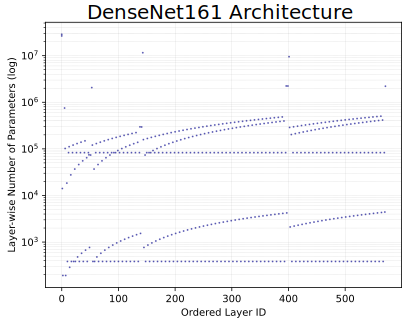
\includegraphics[width=0.5\textwidth]{figures/densenet161_num-params.pdf}
    \caption{Layer-wise Depiction of DenseNet161 parameters.}
    \label{fig:densenet-params}
\end{figure}


% INCLUDE TABLE WITH ALL CORRELATIONS OF TIME vs PARAM

\subsection{Quantitative Evaluation}
To quantitatively evaluate the performance of each CAM visualization and demonstrate the information gained through deeper layers in a CNN, we calculate the Remove and Debias (ROAD) score \cite{Rong22}. This metric has superior computational efficiency and prevents data leakage found with other CAM performance metrics \cite{Rong22}. ROAD perturbs images through noisy linear imputations, blurring regions of the image based on neighbouring pixel values. The confidence increase (or decrease) \textit{C} in classification score using the perturbed image with the least relevant pixels \textit{LRP} (or most relevant pixels \textit{MRP}) is then used to evaluate the accuracy of a CAM visualization. Since the percentage of pixels perturbed affects the ROAD performance, we evaluate ROAD at \textit{p =} 20\%, 40\%, 60\% and 80\% pixel perturbation thresholds. As proposed by Gildenblat \cite{Gildenblat21}, we combine the least relevant pixel and most relevant pixel scores for our final metric: 

\begin{equation}
ROAD(L^c_{CAM(A^{l})}) = \sum\limits_{p} \frac{(C^p_{L_{LRP}} – C^p_{L_{MRP}})}{2}
\end{equation}

A ROAD score is calculated for each CAM generated. Therefore, for \textit{N} differentiable layers in a CNN, there will be \textit{N} ROAD scores calculated for CAManim. We denote this series of ROAD values as the 'yellow brick ROAD', or ybROAD for short.

\begin{equation}\label{eqn:cam-form}
ybROAD = \concat_{l}^{N}ROAD(L^c_{CAM(A^{l})})
\end{equation}

The ybROAD metric can be used to analyze performance of an experiment with given class, image, and CNN model over all layers of the network. In this study, we identify the CNN layer that identifies features with the largest impact on model performance through ybROAD\_{max}. The ybROAD\_{mean} score is also calculated to summarize the overall ROAD performance of a model.

%yellow brick ROAD ... following the path of layers in a CNN

\begin{figure*}
    \centering
    \includegraphics[width=\textwidth]{figures/conceptual-overview.pdf}
    \caption{Conceptual Overview of Generating an Animation of a Resnet's End-to-End Activation Maps for a given Image.}
    \label{fig:overview}
\end{figure*}

% Algorithm here


\section{Results \& Discussion}
In this section, we first define the pre-trained models and datasets used to evaluate CAManim in Section \ref{sec:datamodel}. Next, we demonstrate CAManim in high criticality fields using a ResNet50 model fine-tuned to perform breast cancer classification in Section \ref{sec:bcresnet}. We then show example visualizations from CAManim for 10 different CAM variations in Section \ref{sec:activationmaps} and discuss abnormal visualizations in Section \ref{sec:visissues}. Lastly, we discuss the ybROAD performance of CAManim in Section \ref{sec:ybROAD}.

\subsection{Pre-trained Models and Datasets}
\label{sec:datamodel}
To evaluate CAManim, we use models from TorchVision pre-trained on the 2012 ImageNet-1K dataset.  Specifically, results are shown for AlexNet \cite{}, ConvNext \cite{}, DenseNet161 \cite{}, EfficientNet-b7 \cite{}, MaxViT-t \cite{}, and SqueezeNet \cite{}. The CAManim videos for an additional 14 models can be found here: \url{https://omni-ml.github.io/pytorch-grad-cam-anim/}. All results in this study (apart from the high criticality evaluation) are based on a popular image used in CAM evaluations, preprocessed by resizing to 224 x 224 and normalizing the final image.

Next, we demonstrate the utility of CAManim in high criticality fields. Specifically, we take a ResNet50 model pre-trained on the ImageNet dataset, and fine-tune the model using the Kaggle breast ultrasound data to classify malignant vs normal images \cite{}{}{}. For simplification, we call this network BC-ResNet50 (Breast Cancer -ResNet50). This dataset consists of 133 normal images and 210 malignant images, which are split into a 80-10-10\% train-validation-test split. Images are preprocessed to a size of 224 x 224 and augmentations are applied to the training set. Preprocessing and training steps are selected based on MONAI recommendations \cite{}. After fine-tuning the network, CAManim is run with an example test image of the malignant class to understand how the CNN makes a correct prediction of cancer. 

\subsection{Case Study: End-to-End BC-ResNet50 Visualization for Malignant Tumour Prediction}
\label{sec:bcresnet}

Figure \ref{fig:mednet-viz} illustrates the layerwise activations that BC-ResNet50 considers when determining the 
`malignant' tumour.

\begin{figure*}
    \centering
    \includegraphics[width=\textwidth]{figures/mednet-10percentile_final.pdf}
    \caption{Visualization of the activation maps from BC-ResNet50 to visually depict how the model predicts the 'malignant' tumour class. Only the 10th percentile layers are illustrated for concision.}
    \label{fig:mednet-viz}
\end{figure*}

\subsection{Visualizing End-to-End Network Activation Maps}
\label{sec:activationmaps}

We demonstrate the performance of CAManim on 10 different CAM methods, including seven gradient-based methods (EigenGradCAM, GradCAM, GradCAMElementWise, GradCAM++, HiResCAm, LayerCAM, and XGradCAM), two perturbation methods (AblationCAM and ScoreCAM), a principal components method (EigenCAM), and RandomCAM. RandomCAM generates random feature activation maps from a uniform distribution between -1 and 1.

\begin{figure*}
    \centering
    \includegraphics[width=\textwidth]{figures/bear_one-model-all-cams_final.pdf}
    \caption{End-to-End Activation Map Visualization for 10 CAMs using DenseNet161. Every 10th percentile map is depicted, from left to right.}
    \label{fig:all-cams}
\end{figure*}


\begin{figure}
    \centering
    \includegraphics[width=0.5\textwidth]{figures/bear_one-cam-all-models_final.pdf}
    \caption{Initial, middle, and final activation maps applying a single CAM, HiResCAM, to various model architechtures.}
    \label{fig:my_label}
\end{figure}

\subsection{Layer-Type Visualization Issues}
\label{sec:visissues}

Certain differentiable layers may produce unanticipated CAM visualizations, as depicted in Figure \ref{fig:bad_layers}. In these layers, images are compressed to 1-dimensional (1D) representation, preventing valid 2D features from being discovered through CAM formulations. Instead, individual neurons that are highly activated show up as vertical or horizontal lines over the image. While these images are not informative, they are not incorrect; they simply depict visualizations of 1D layers.

\begin{figure}
    \centering
    \includegraphics[width=0.4\textwidth]{figures/bad_layers.png}
    \caption{Visualization of CAManim for fully connected and average pooling layers.}
    \label{fig:bad_layers}
\end{figure}

\subsection{ybROAD Quantitative Evaluation}
\label{sec:ybROAD}

Figure X(YBROAD) displays the ybROAD for X trials of generating CAManim for the bear image using ResNet152. Initially, the individual-layer ROAD performance is very high ($\sim$0.45). At this point, the CNN layer is activating many small regions throughout the image; when each of these areas is perturbed, it is difficult to correctly classify the image, and the ROAD score increases. As the network starts learning larger features, less of the bear image is perturbed, and the ROAD score decreases. Towards the end of the network, the ROAD score increases again as the small activations are combined together to cover the entire bear. This demonstrates how the ybROAD score can provide additional information on how the network is learning. %information about max and mean?? max chooses best image?

%lets you choose which image is most accurate

\section{Conclusion}
The conclusion goes here. this is more of the conclusion

% use section* for acknowledgement
\section*{Acknowledgment}
The authors would like to thank...
more thanks here

\bibliographystyle{IEEEtran}
\bibliography{references} 
% that's all folks
\end{document}


